\documentclass[12pt]{article}
\usepackage[utf8]{inputenc}

\usepackage{fullpage}
\usepackage{graphicx}
\usepackage{amsthm}
\usepackage{tikz}
\usepackage[spanish]{babel}

\newtheorem{definition}{Definición}
\newtheorem{lemma}{Proposición}



\begin{document}
\section{Fundamentos te\'{o}ricos}
\subsection{Los puentes de K\"{o}nigsberg}
\begin{center}
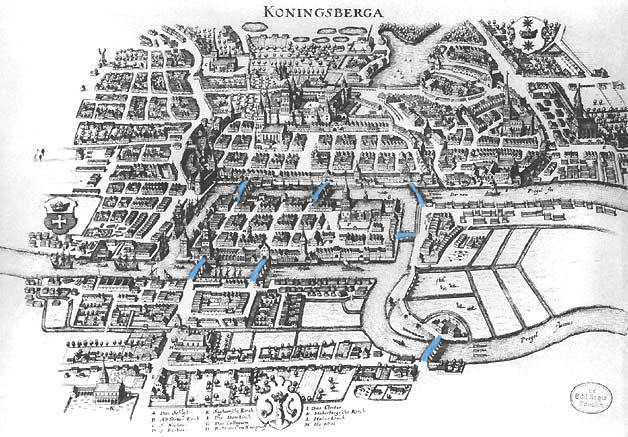
\includegraphics[scale=0.5]{koenigsberg.jpg}
\end{center}
El problema de los puentes de K\"{o}nigsberg ha generado interrogantes en los matemáticos del siglo 18. La meta es de encontrar un camino que vaya por la ciudad, cruzando exactamente una vez cada uno de los siete puentes y terminar el recorrido en el mismo lugar donde comenzó. En 1736 este problema es resuelto por el matemático suizo Leonard Euler, que en ese momento era profesor de matemática en la universidad de San Petersburgo. Euler logró demostrar, que dicho camino no puede existir.
\subsubsection{Euler y el problema de los puentes de K\"{o}nigsberg}
Al buscar un camino cíclico, el cual cruce los siete puentes de K\"{o}nigsberg exactamente una vez, escribe Euler que una forma de resolver el problema, era trazar todos los caminos posibles y revisar si alguno de ellos tiene las características deseadas. Esta solución es demasiado trabajosa para problemas más complejos, por lo cual Euler quería desarrollar un método matemático que le indique si un camino así sería posible. Primero simplificó el mapa de K\"{o}nigsberg, tal que la secuencia de letras A,B,C y D pueda describir cada camino posible por la ciudad.
\begin{center}
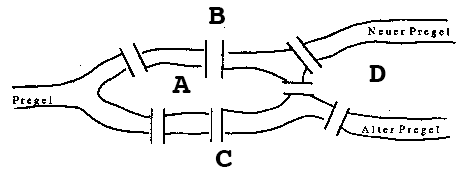
\includegraphics[scale=0.7]{pregelbruecken.png}
\end{center}
Por ejemplo, la secuencia $ADCABAC$ describe el camino que comienza en A, cruza el puente para llegar a $D$, va de $D$ a $C$, etc. Este camino cruza seis de los siete puentes, los cuales pueden ser descritos como los pares $AD$, $DC$, $CA$, $AB$, $BA$ y $AC$. Esto simplifica el problema, ya que solamente se tiene que encontrar una secuencia de 8 letras (ya que se trata de 7 puentes), en la que cada letra aparezca en relación a la cantidad de puentes que la conecta. Antes de buscar esa secuencia, Euler quería demostrar que existe. Euler argumenta que $D$ tiene que aparecer exactamente dos veces en esa secuencia, ya que $D$ está conectado con tres puentes. Si $D$ aparece una vez en la secuencia, solamente se cruzarían dos de los tres puentes. Si $D$ aparece tres veces en la secuencia, debería estar conectado con, como mínimo, cuatro puentes. Asimismo deberían aparecer $C$ y $B$ dos, y $A$ tres veces. Por lo tanto, la secuencia necesitaría 9 letras, lo que es imposible, ya que solamente hay 7 puentes. Esto demuestra que un camino que cruce cada puente un a sola vez y que termine en la letra que comenzó, no existe. 
\\A partir de la solución a este problema Euler establece los fundamentos para la teoría de los grafos a pesar de que no utilizó conceptos como vértices, aristas o grafos.
\subsection{Caminos y grafos eulerianos}
\begin{definition}
Un camino $C$ en un grafo conexo $G$ se le denomina \emph{camino euleriano}, cuando cada arista de $G$ se encuentra en $C$.
\end{definition}
\begin{definition}
Un grafo conexo $G$ se le denomnia \emph{grafo euleriano}, cuando contiene un camino euleriano cerrado. Un camino euleriano cerrado se le llama ciclo euleriano.
\end{definition}
\begin{lemma}
Sea un grafo conexo $G$ con los siguientes atributos:
\begin{enumerate}
\item $G$ es un grafo euleriano.
\item Cada nodo de $G$ tiene un grado par.
\item Las aristas de $G$ se pueden separar en ciclos disjuntos.
\end{enumerate}
\end{lemma}
\begin{proof}
La proposición es demostrada mediante el razonamiento circular.
\\$1. \rightarrow 2.$
\\Asumimos que $G$ contenga un ciclo euleriano $C$. Sea $v$ un nodo cualquiera de $G$. Cada vez que $C$ pase por $v$, tiene que pasar por dos aristas incidentes a $v$. Si cada arista incidente a $v$ es recorrida por $C$, entonces el grado de $v$ es par.
\\$2. \rightarrow 3.$
\\Asumimos que el grado cada nodo $v \in G$ es par. Ya que $G$ es un grafo conexo y ningún nodo tiene un grado de 1, entonces $G$ no es un árbol y, por lo tanto, tiene por lo menos un ciclo. Tiene $G$ exactamente un ciclo, entonces es $G$ un grafo ciclo $C_{n}$ para un $n$ y la disyunción seria solo ese ciclo. Suponiendo que sea verdadero para grafos que no contengan mas de $k$ ciclos y $G$ contiene $k+1$ ciclos. Sea $C$ un ciclo en $G$ y sea $G'$ el grafo resultante de $G$, cuando se eliminan las aristas pertenecientes a $C$. Al eliminar las aristas de $C$, el grado de cada nodo se reduce por 2. Por lo tanto, el grado de cada nodo de $G'$ es par. De esto resulta, que a cada componente conexo de $G'$, no le pertenecen mas de $k$ ciclos. Cada componente conexo de $G'$ cumple con la suposición.
\\$3. \rightarrow 1.$
\\Asumimos que la disyunción de $G$ sean ciclos. Estos ciclos se llamarán $S_{1}, S_{2}, ..., S_{k}$. Sea $C$ el ciclo mas largo, tal que el conjunto de aristas de $C$ es $$E(C)=E(S_{j1}) \cup E(S_{j2}) \cup ... \cup E(S_{jm})$$ para varias $S_{j1}, S_{j2}, ..., S_{jm}$. Sea entonces $e$ una arista que no pertenezca a $C$, pero que sea incidente en un nodo $v$ de $C$, entonces $e$ y $v$ deberían pertenecer a un ciclo que no comparte ninguna arista con $C$. Sea entonces $C'$ el ciclo que se obtiene uniendo $C$ y $S_{i}$ en $v$. Como a $C'$ le pertenecen todas las aristas de $C$ y $S_{i}$, contradice que $C$ sea el ciclo mas largo. Por lo tanto ya le perteneces todas las aristas de $G$ a $C$, lo que quiere decir que $C$ es un ciclo euleriano. Por ello, $G$ es un grafo euleriano.
\end{proof}
\subsection{Algoritmos para encontrar ciclos eulerianos}
Si se conoce que $G$ es un grafo euleriano, se tiene que poder encontrar el ciclo euleriano en $G$. Esto es posible con el algoritmo de Hierholzer.
\subsubsection{Algoritmo de Hierholzer}
Sea dado un grafo euleriano $G$
\begin{enumerate}
\item Encuentre un ciclo en $G$, ll\'{a}melo $R_{1}$ y marque sus aristas. Sea i=1.
\item Si $R_{i}$ contiene todas las aristas de $G$, entonces es $R_{i}$ el ciclo euleriano.
\item Si $R_{i}$ no contiene todas las aristas de $G$, sea $v_{i}$ un nodo en $R_{i}$, en el cual incide una arista $e_{i}$ que no esta marcada.
\item Encuentre un ciclo $Q_{i}$, de aristas no marcadas, que contenga tanto $v_{i}$ como $e_{i}$. Marque las aristas de $Q_{i}$.
\item Cree un nuevo ciclo $R_{i+1}$, uniendo $R_{i}$ y $Q_{i}$ en $v_{i}$.
\item Eleve i por 1 y continúe con el paso 2.
\end{enumerate}
Que el resultado del algoritmo de Hierholzer es un ciclo euleriano, se deja deducir a partir de la condición 3 de la proposición 1.
\begin{definition}
Sea $G$ un grafo y $e \in E(G)$. Si al eliminar $e$ crece el numero de componentes de $G$, entonces a $e$ se le denomina como puente de $G$.
\end{definition}
\subsubsection{Algoritmo de Fleury}
Sea $G$ un grafo euleriano, en cual ninguna de las aristas estén marcadas.
\begin{enumerate}
\item Elija un nodo y marque ese nodo como "nodo principal".
\item Si todas las aristas de $G$ están marcadas, termino el algoritmo. De lo contrario, siga con el paso 3.
\item Elija una arista no marcada incidente al "nodo principal". Si es posible, una que no sea un puente en el subgrafo de $G$, que esta compuesto de las aristas no marcadas. Si no es posible, elija cualquier arista incidente en el "nodo principal". Marque la arista elegida y marque al otro nodo incidente de la arista como el nuevo "nodo principal".
\item Siga al paso 2.
\end{enumerate}
Para demostrar que el resultado del algoritmo de Fleury es un ciclo euleriano, se tiene que observar el caso en el que el algoritmo se puede quedar atascado.
\begin{proof}
Ya que el grado de cada nodo de $G$ es par, podemos salir de cada nodo, con la excepción del nodo de inicio $v$. Supongamos que el algoritmo se atasque en el nodo $v$. Las aristas no marcadas forman componentes conexas, las cuales son eulerianas, ya que el grado de cada nodo es par. Si el ultimo nodo visitado por el algoritmo es $w$ y luego salio por la arista $wv_{1}$, entonces el resto del camino se define por $v_{1}v_{2}...v_{k}=v$. Esto demuestra que la arista $wv_{1}$ es un puente en el algoritmo de Fleury. Sin embargo existen por lo menos dos aristas incidentes en $w$, que no son puentes. Por eso la arista $wv_{1}$ desde un principio no es seleccionada por el algoritmo.
\end{proof}
A diferencia del algoritmo de Hierholzer, es posible, mediante el algoritmo de Fleury, de encontrar un camino euleriano, en grafos con dos nodos de grado impar. Para ello se elije uno de los dos nodos como "nodo principal".
\newpage
\section{Estructura del programa}
\subsection{Algoritmo para generar la matriz de relaci\'{o}n}
\begin{enumerate}
\item Sea el ingreso del usuario $m$, tal que $6\leq m\leq 12$.
\item Se genera la matriz de relaci\'{o}n $M_{R}$ de $m \times m$.
\item A todos los elementos de $m_{ij}$ de $M_{R}$, tal que $i=j$, se les asigna el valor $0$.
\item Sea $i=1$.
\item A cada uno los valores $m_{ij}$, en los que $j>i$, se les asigna un valor de $1$ o $0$, de tal manera que la suma de los elementos de $i$ que contengan $1$ sea par.
\item $m_{ij}=m_{ji}$, para todos los elementos de la fila $i$, para los que vale $j>i$.
\item Si $i=m-1$, termina el algoritmo. De lo contrario aumenta el valor de $i$ por uno y se regresa al paso 5.
\end{enumerate}
\subsubsection*{Ejemplo}
Si el ingreso del usuario es $m=7$, se genera una matriz de relaci\'{o}n $M_{R}$ (para los nodos $A, B, C, ..., G$) de $7\times 7$. La matriz resultante del paso 3 ser\'{i}a esta:
$$M_{R}=
\bordermatrix{
     &     A     &     B          &     C          &     D          &     E          &     F          &     G          \cr
A    &     0     &     m_{AB}     &     m_{AC}     &     m_{AD}     &     m_{AE}     &     m_{AF}     &     m_{AG}     \cr
B    &     m_{BA}&     0          &     m_{BC}     &     m_{BD}     &     m_{BE}     &     m_{BF}     &     m_{BG}     \cr
C    &     m_{CA}&     m_{CB}     &     0          &     m_{CD}     &     m_{CE}     &     m_{CF}     &     m_{CG}     \cr
D    &     m_{DA}&     m_{DB}     &     m_{DC}     &     0          &     m_{DE}     &     m_{DF}     &     m_{DG}     \cr
E    &     m_{EA}&     m_{EB}     &     m_{EC}     &     m_{ED}     &     0          &     m_{EF}     &     m_{EG}     \cr
F    &     m_{FA}&     m_{FB}     &     m_{FC}     &     m_{FD}     &     m_{FE}     &     0          &     m_{FG}     \cr
G    &     m_{GA}&     m_{GB}     &     m_{GC}     &     m_{GD}     &     m_{GE}     &     m_{GF}     &     0     \cr
}
$$
Al culminar el bucle del algoritmo por primera vez, es esta la matriz:
$$M_{R}=
\bordermatrix{
     &     A     &     B          &     C          &     D          &     E          &     F          &     G          \cr
A    &     0     &     1          &     1          &     0          &     1          &     0          &     1          \cr
B    &     1     &     0          &     m_{BC}     &     m_{BD}     &     m_{BE}     &     m_{BF}     &     m_{BG}     \cr
C    &     1     &     m_{CB}     &     0          &     m_{CD}     &     m_{CE}     &     m_{CF}     &     m_{CG}     \cr
D    &     0     &     m_{DB}     &     m_{DC}     &     0          &     m_{DE}     &     m_{DF}     &     m_{DG}     \cr
E    &     1     &     m_{EB}     &     m_{EC}     &     m_{ED}     &     0          &     m_{EF}     &     m_{EG}     \cr
F    &     0     &     m_{FB}     &     m_{FC}     &     m_{FD}     &     m_{FE}     &     0          &     m_{FG}     \cr
G    &     1     &     m_{GB}     &     m_{GC}     &     m_{GD}     &     m_{GE}     &     m_{GF}     &     0     \cr
}
$$
Una vez culminado el algoritmo, se obtiene la matriz de relaci\'{o}n
$$M_{R}=
\bordermatrix{
 &A&B&C&D&E&F&G\cr
A&0&1&1&0&1&0&1\cr
B&1&0&1&0&0&0&0\cr
C&1&1&0&0&1&1&0\cr
D&0&0&0&0&1&0&1\cr
E&1&0&1&1&0&1&0\cr
F&0&0&1&0&1&0&0\cr
G&1&0&0&1&0&0&0\cr
}
$$
\subsection{Algoritmo para dibujar el grafo correspondiente a $M_{R}$}
\begin{enumerate}
\item Se dibujan los nodos $N_{1}, N_{2}, ..., N_{m}$ al rededor de un punto central, comenzando por $N_{1}$ en $0^{\circ}$.
\item Se selecciona el grado de separaci\'{o}n $\alpha$, de tal manera que para cualquier $N_{n}$, $$\alpha(N_{n}) = n\frac{360^{\circ}}{m}$$
\item Para cada $m_{ij}\in <M_{R}  \vert  i>j$ que sea 1, se traza una arista del nodo $N_{i}$ al nodo $N_{j}$.
\end{enumerate}
\subsubsection*{Ejemplo}
Dibujaremos el grafo a partir de la matriz dada en el ejemplo anterior. \\Tomamos al nodo $A$ como nuestro $N_{1}$.  Como $m = 7$, el grado de la separaci\'{o}n de cada nodo al nodo previo es de $\alpha \approx 51^\circ$. La imagen resultante ser\'{i}a la siguiente:\\
\begin{center}
\begin{tikzpicture}
\draw (0:3cm) circle (0.3cm) node(a){A};
\draw (51:3cm) circle (0.3cm) node (b)      {B};
\draw (102:3cm) circle (0.3cm) node(c)     {C};
\draw (153:3cm) circle (0.3cm) node(d)     {D};
\draw (204:3cm) circle (0.3cm) node(e)     {E};
\draw (255:3cm) circle (0.3cm) node(f)     {F};
\draw (306:3cm) circle (0.3cm) node(g)     {G};
\draw[dashed, very thick] (0,0) -- (a) (0,0) -- (b);
\draw (1,0) arc (0:51:1cm) node [right, near start] {$51^\circ$};
\end{tikzpicture}
\end{center}
\newpage
Al conectar los nodos con aristas seg\'{u}n $M_{R}$, se obtiene el grafo completado.
\begin{center}
\begin{tikzpicture}
\draw (0:3cm) circle (0.3cm) node(a){A};
\draw (51:3cm) circle (0.3cm) node (b)      {B};
\draw (102:3cm) circle (0.3cm) node(c)     {C};
\draw (153:3cm) circle (0.3cm) node(d)     {D};
\draw (204:3cm) circle (0.3cm) node(e)     {E};
\draw (255:3cm) circle (0.3cm) node(f)     {F};
\draw (306:3cm) circle (0.3cm) node(g)     {G};
\draw [very thick] (a) -- (b) (a) -- (c) (a) -- (e) (a) -- (g);
\draw [very thick] (b) -- (c);
\draw [very thick] (c) -- (e) (c) -- (f);
\draw [very thick] (d) -- (e) (d) -- (g);
\draw [very thick] (e) -- (f);
\end{tikzpicture}
\end{center}
\end{document}
